\chapter{Experimental Results and Analysis}

\section{Benchmarking Setup}

To evaluate the performance of selected tracking algorithms in underwater environments, we conducted benchmarking experiments on the UOT100 dataset using the GOT-10k toolkit. Six trackers were implemented or integrated via OpenCV, including classical correlation filter-based methods (MOSSE, KCF), regression and transformer-based neural models (GOTURN, ViT), and modern deep learning methods based on Siamese architectures (DaSiamRPN, NanoTrack). All experiments were run on the same machine to ensure consistency in evaluation. The primary performance metrics include Average Overlap (AO), Success Rate (SR), Success Curve, and runtime efficiency in terms of frames per second (FPS).


\section{Quantitative Results}

While the success curve provides an overall picture of tracking accuracy across different thresholds, it is also essential to compare the numerical values of Average Overlap (AO), Success Rate (SR), Frames Per Second (FPS), and GPU usage to evaluate both the accuracy and the practicality of each tracker.

Table~\ref{tab:ao_sr_fps_gpu_summary} summarizes these metrics for each evaluated tracker:
\begin{table}[ht]
    \centering
    \begin{tabular}{lcccc}
        \toprule
        \textbf{Tracker} & \textbf{AO} & \textbf{SR} & \textbf{FPS} & \textbf{Hardware Used} \\
        \midrule
        NanoTrack & 0.510 & 0.572 & 90.29 & GPU Quadro T1000 \\
        DaSiamRPN & 0.402 & 0.470 & 72.09 & GPU Quadro T1000 \\
        KCF & 0.266 & 0.310 & 64.87 & CPU Intel Core i7-9th \\
        MOSSE & 0.266 & 0.305 & 150.98 & CPU Intel Core i7-9th \\
        ViT & 0.258 & 0.299 & 70.58 & GPU Quadro T1000 \\
        GOTURN & 0.136 & 0.180 & 25.59 & GPU Quadro T1000 \\
        \bottomrule
    \end{tabular}
    \caption{Summary of AO, SR, FPS, and hardware usage for all evaluated trackers.}
    \label{tab:ao_sr_fps_gpu_summary}
\end{table}

Several conclusions can be drawn from this data:

\begin{itemize} \item \textbf{NanoTrack} achieves the best trade-off between speed and accuracy, making it well-suited for real-time underwater applications on modern GPUs. \item \textbf{MOSSE} is the fastest tracker and does not require a GPU, making it ideal for CPU-only embedded systems, though its accuracy remains limited. \item \textbf{ViT} and \textbf{GOTURN} underperform in AO and SR despite using deep learning, suggesting that they may require domain-specific adaptation to perform well in underwater environments. \end{itemize}


\section{Success Curve Visualization}

Figure~\ref{fig:success_curve} illustrates the success curves for the evaluated trackers on the UOT100 dataset. The curves depict the success rate as a function of the overlap threshold (IoU), ranging from 0 to 1. The legend includes the AO (Average Overlap) for each tracker, providing a concise summary of their overall performance.

\begin{figure}[ht]
    \centering
    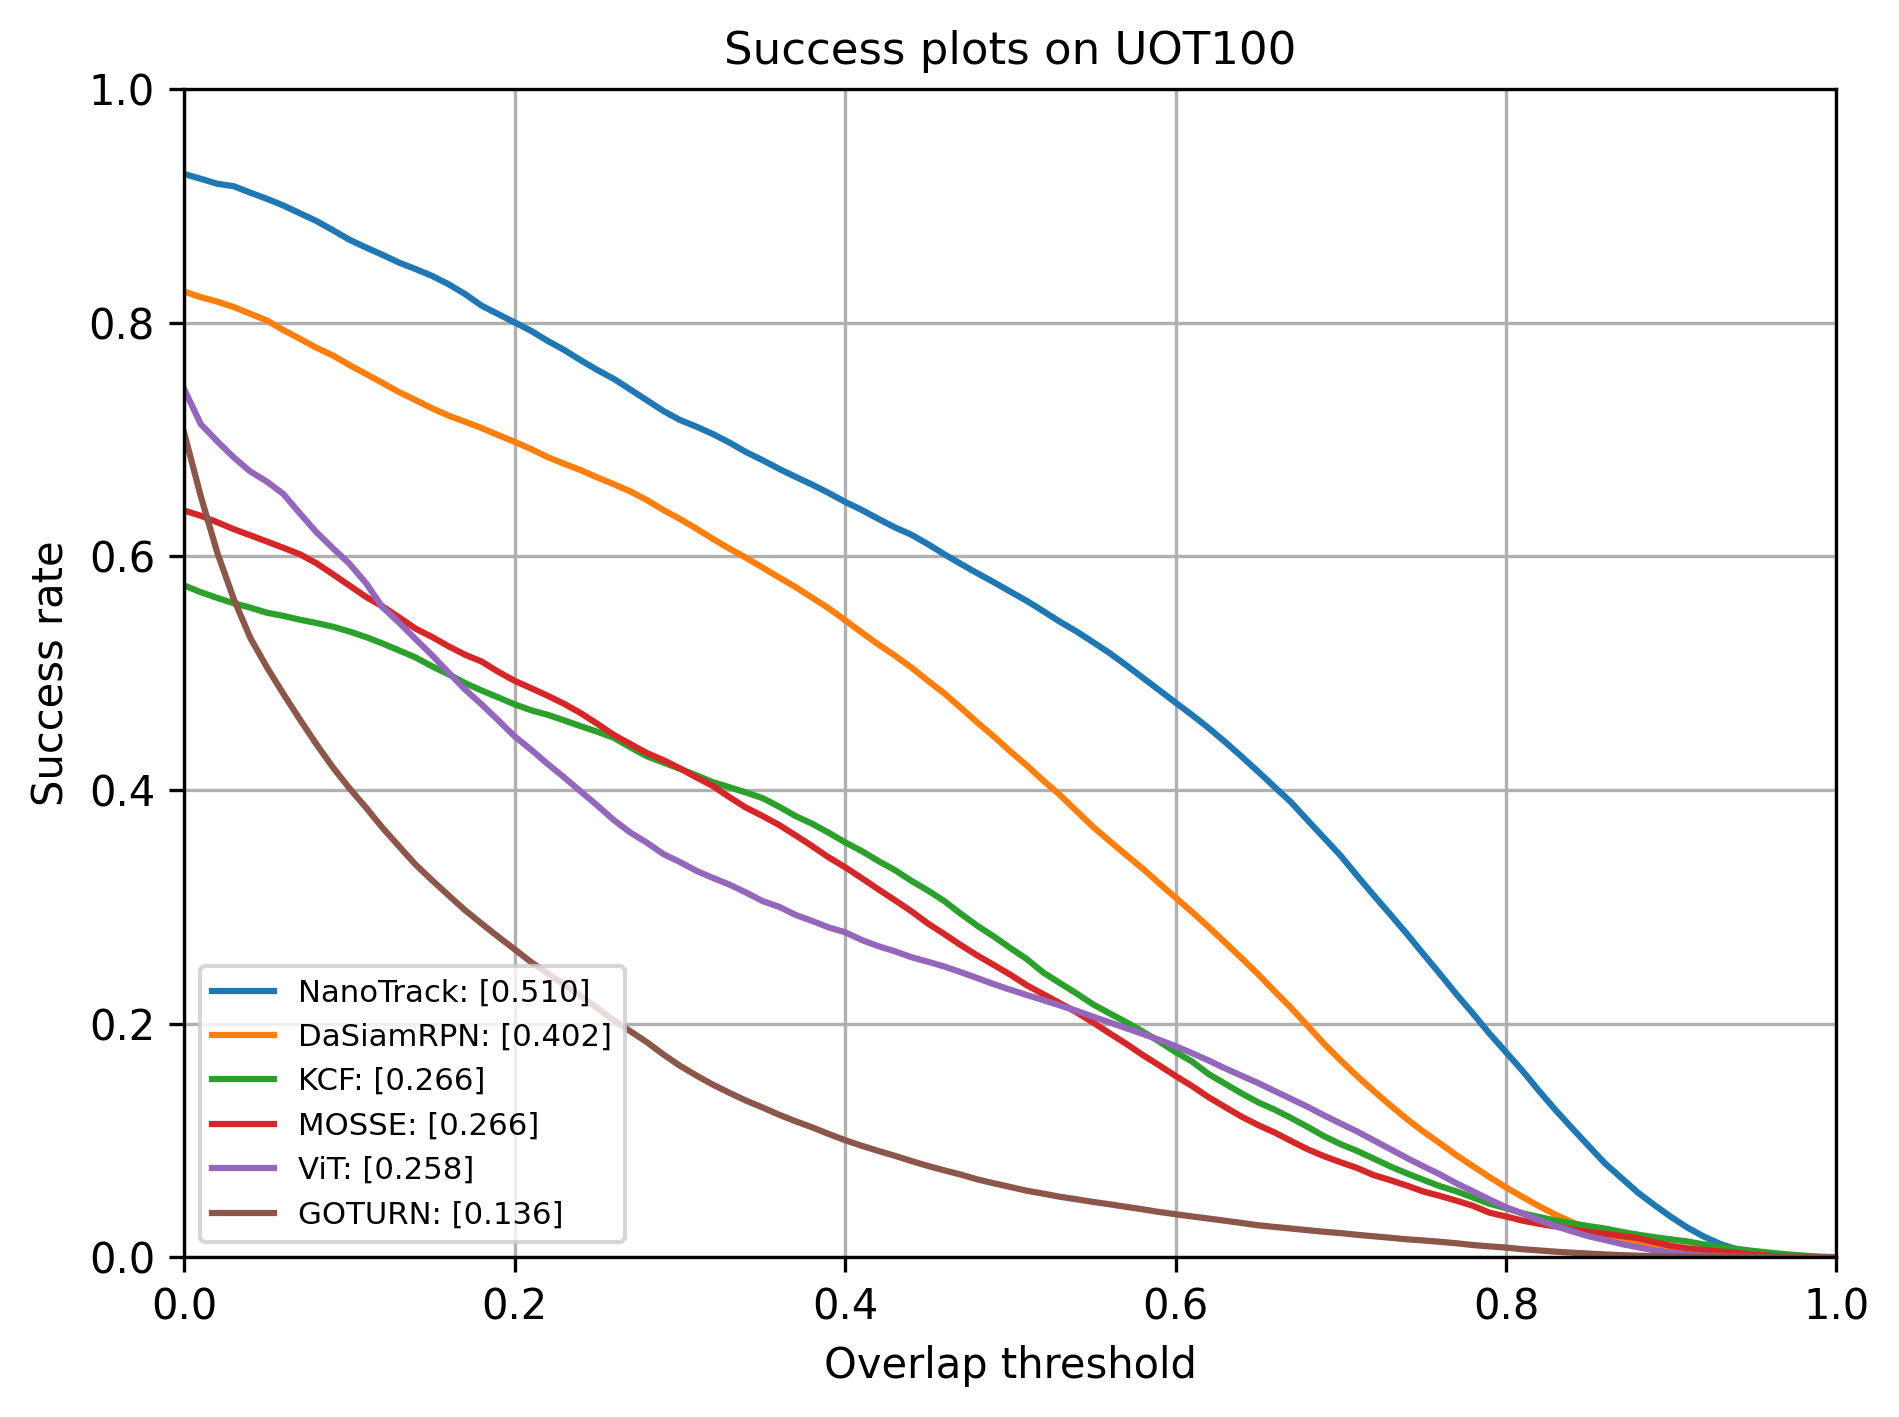
\includegraphics[width=1\textwidth]{images/success_plot.png}
    \caption{Success curves of the evaluated trackers on the UOT100 dataset. The X-axis represents the overlap threshold (IoU), and the Y-axis represents the success rate. The AO (Average Overlap) for each tracker is shown in the legend.}
    \label{fig:success_curve}
\end{figure}

From the success curves, the following observations can be made:
\begin{itemize}
    \item \textbf{NanoTrack} demonstrates stable performance even at higher IoU thresholds (IoU > 0.6), indicating its robustness in challenging scenarios.
    \item The gap between \textbf{NanoTrack} and other trackers widens as the IoU threshold increases, highlighting its superior accuracy.
    \item \textbf{DaSiamRPN} also performs well at moderate thresholds but shows a decline at higher IoU values compared to NanoTrack.
    \item Classical trackers like \textbf{KCF} and \textbf{MOSSE} exhibit limited performance, with success rates dropping significantly at higher thresholds.
    \item \textbf{GOTURN} has the lowest success rate across all thresholds, reflecting its difficulty in adapting to underwater conditions.
\end{itemize}

\section{Qualitative Analysis and Observations under Key Underwater Challenges}

The qualitative analysis of the tracking results provides valuable insights into the strengths and weaknesses of each tracker in various underwater scenarios. The following subsections highlight specific challenges encountered during the evaluation and how different trackers responded to these challenges.

\subsubsection{Low Contrast and Color Attenuation}
One of the most challenging conditions for underwater tracking arises when the target exhibits low contrast against the surrounding background. This often occurs due to color attenuation and uneven lighting, where the object's color becomes similar to that of the background, making it difficult to distinguish and track. Sequences labeled with keywords such as bluelike and greenlike in the UOT100 dataset frequently demonstrate this issue.

\begin{figure}[ht]
    \centering
    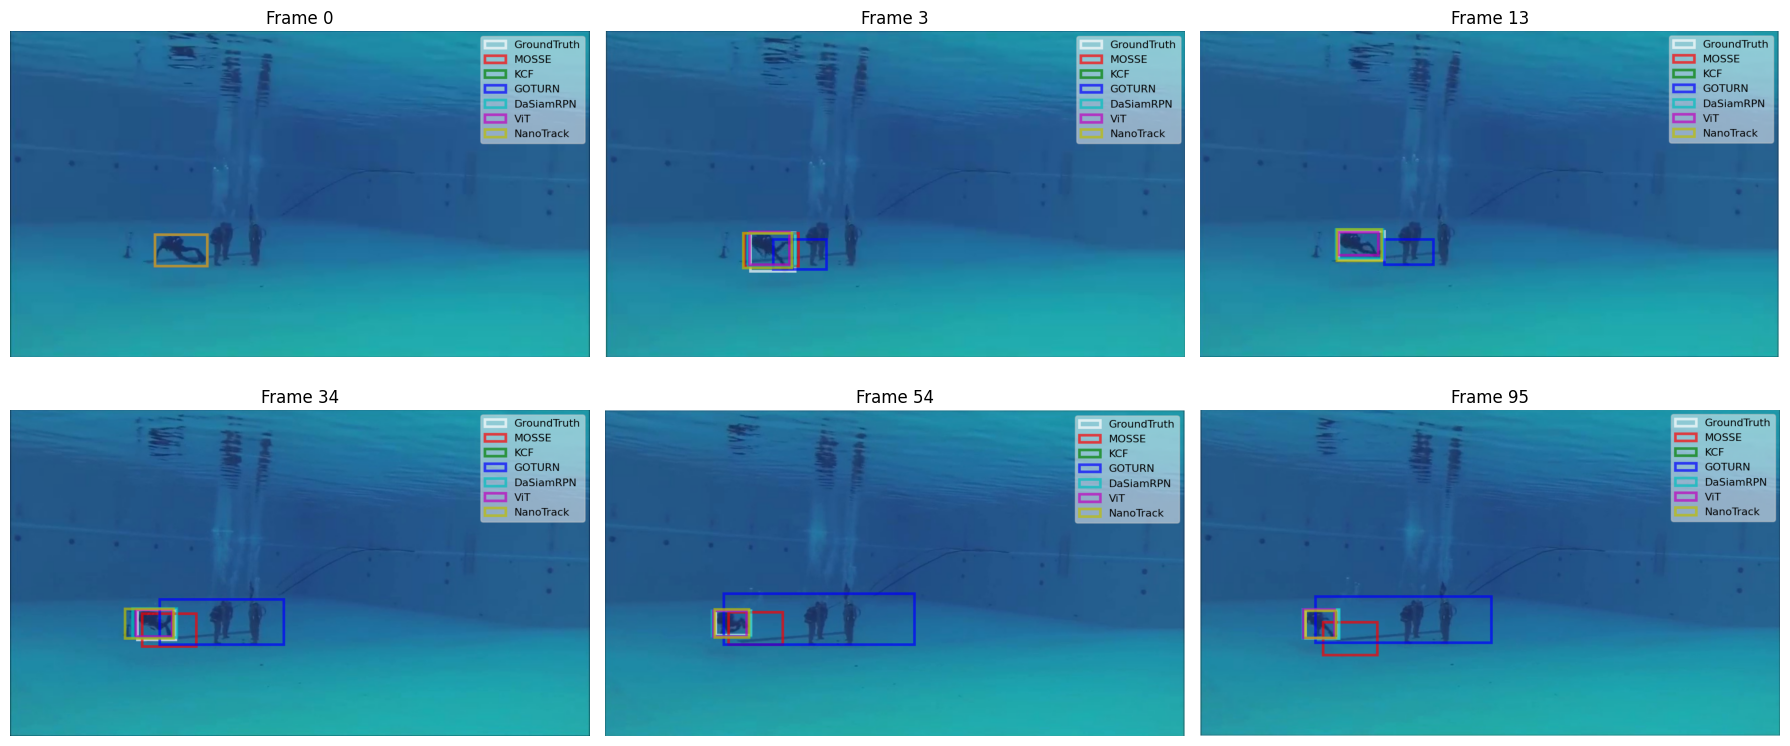
\includegraphics[width=1\textwidth]{images/ArmyDiver3.png}
    \caption{Tracking results of various trackers on a sequence with a diver blurred and having colors similar to the background.}
    \label{fig:low_contrast_example}
\end{figure}

As illustrated in Figure~\ref{fig:low_contrast_example}, this scenario presents considerable difficulty for many trackers. Classical trackers such as KCF tend to lose the target in frames with significant blur or poor contrast. MOSSE, despite its initial success, often fails to maintain consistent tracking once the object becomes visually indistinct from its surroundings. GOTURN, a deep learning-based tracker, also struggles under these conditions—frequently confusing the object with larger regions of the background due to its limited robustness to contrast variations.

In contrast, ViT, NanoTrack, and DaSiamRPN exhibit superior performance in this challenging environment. These trackers are more capable of leveraging deep feature representations to maintain target identity even when the visual signal is weak or ambiguous. Notably, NanoTrack and DaSiamRPN maintain stable tracking across the sequence, demonstrating strong resilience to low contrast and background similarity.

\subsubsection{ Motion Blur and Turbidity}

Another significant challenge in underwater object tracking is the presence of motion blur and turbidity, which often arise due to fast-moving objects, rapid water currents, or camera instability. These factors can lead to severe blurring of the target, making it difficult for trackers to maintain accurate localization.

\begin{figure}[ht]
    \centering
    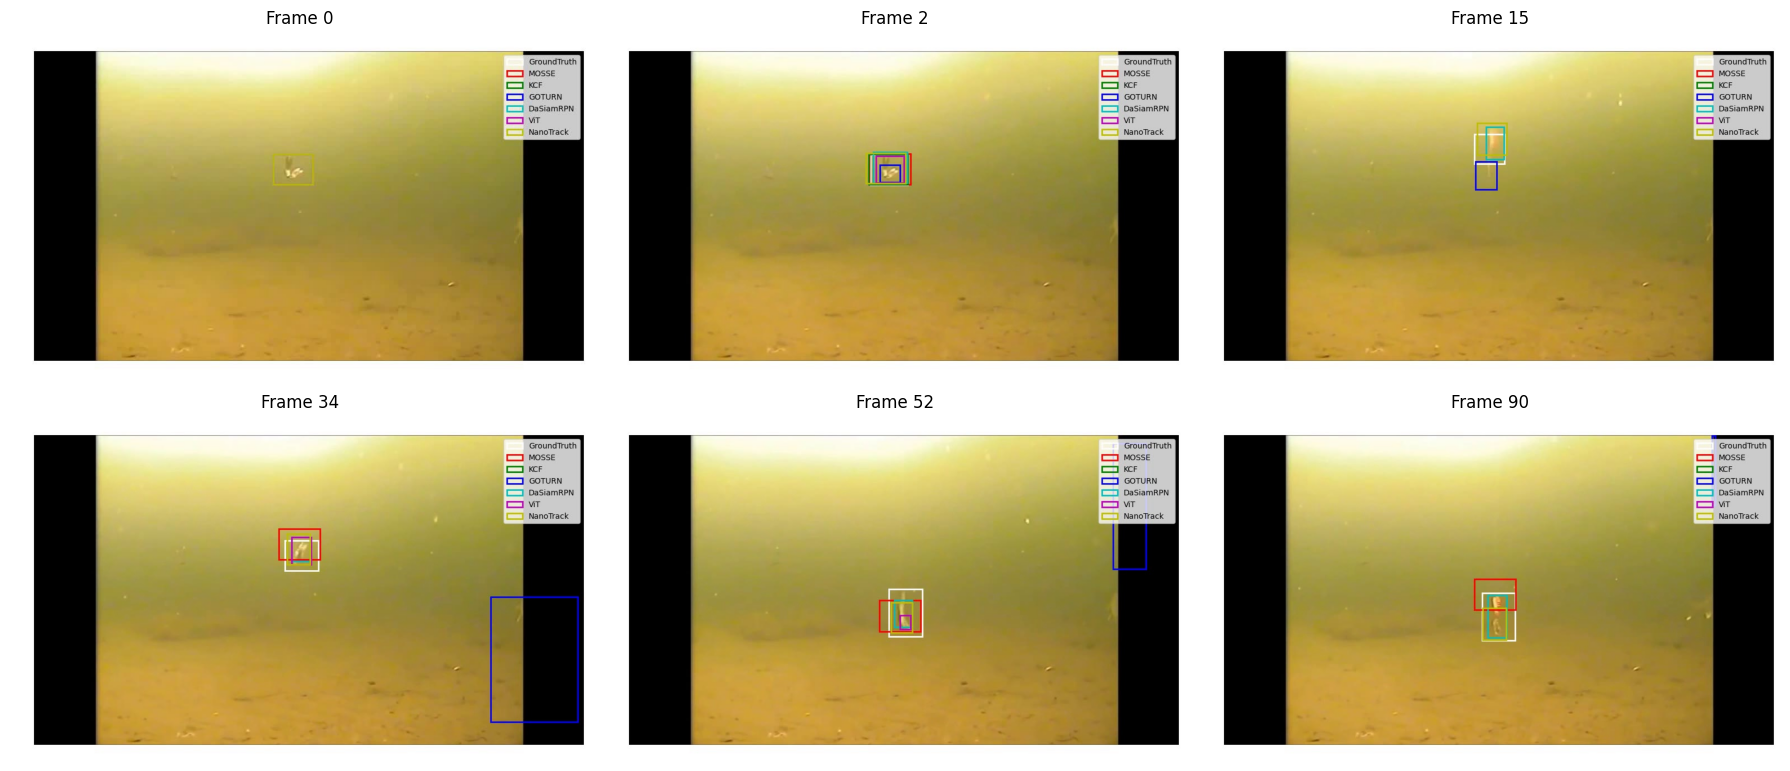
\includegraphics[width=1\textwidth]{images/FishingBait.png}
    \caption{Tracking results on a sequence featuring a fast-moving fishing bait with low contrast against the background.}
    \label{fig:motion_blur_example}
\end{figure}

As shown in Figure~\ref{fig:motion_blur_example}, most trackers are initially able to detect and follow the object in the early frames. However, as the fishing bait accelerates, many trackers quickly lose the target due to motion blur and reduced visibility. Among the evaluated trackers, DaSiamRPN demonstrates the most consistent performance, maintaining a stable lock on the target throughout the sequence.

ViT also shows promising results, particularly in its ability to re-detect the object once the bait slows down and becomes clearer. Nevertheless, its initial tracking during the high-speed movement phase is less reliable. In contrast, other trackers—including classical methods and some deep learning-based models—fail to recover the object once tracking is lost.

These results indicate that DaSiamRPN is especially well-suited for scenarios involving fast object motion and blurry frames, likely due to its strong feature representation and robust region proposal mechanism.

\subsubsection{Occlusion and Similar-looking Distractors}

Occlusion is a common and challenging scenario in underwater tracking, where the target is temporarily blocked by other objects such as marine animals, plants, or underwater structures. The difficulty is further amplified when the occluding objects share similar visual characteristics with the target, creating distractors that can mislead the tracker.

\begin{figure}[ht]
    \centering
    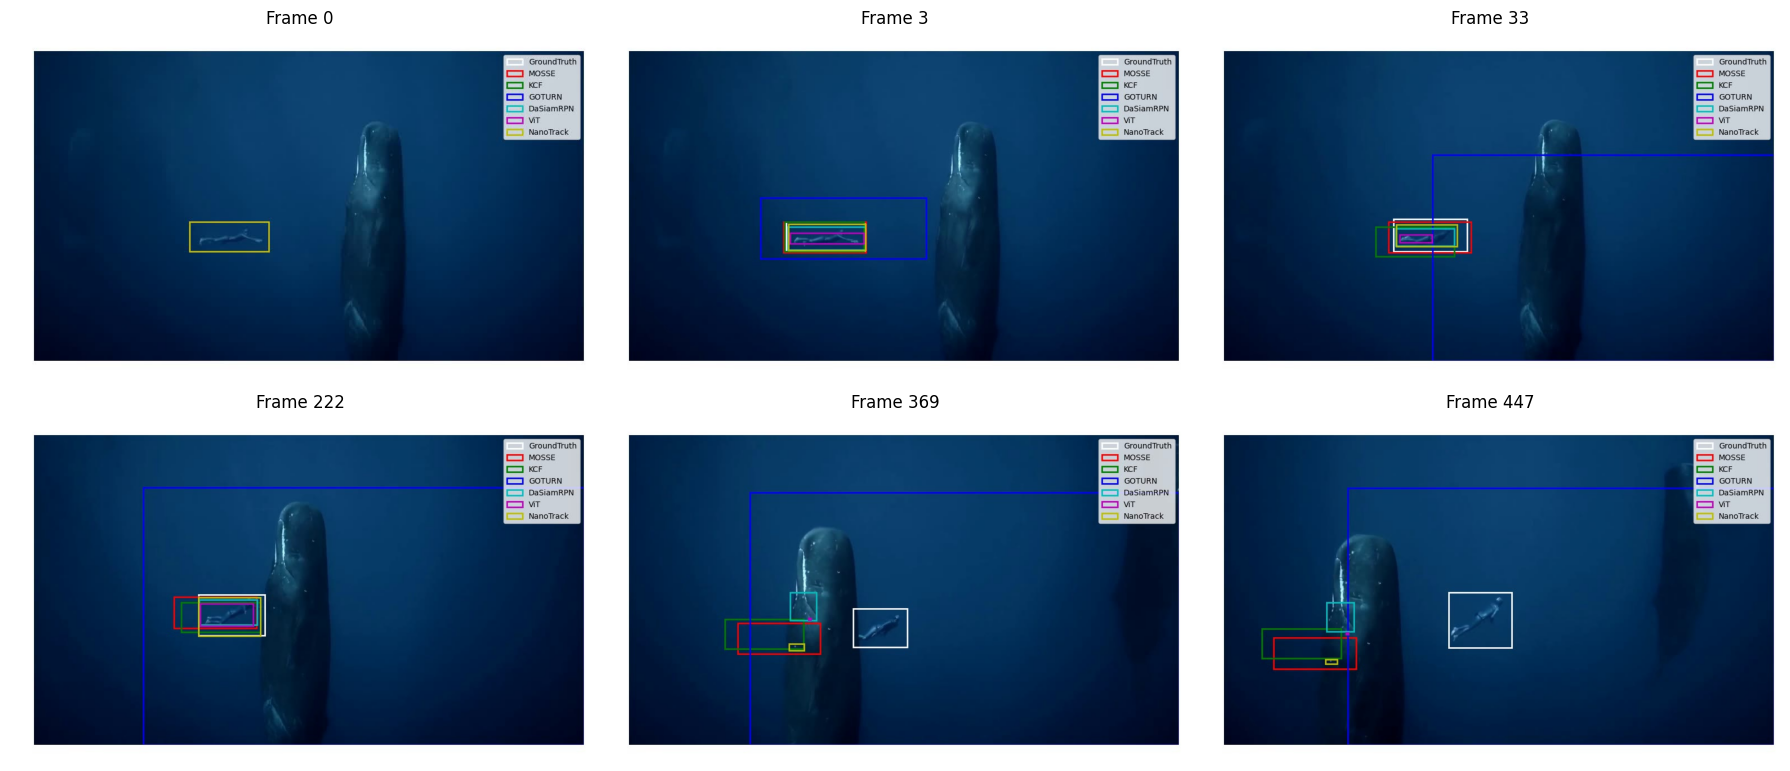
\includegraphics[width=1\textwidth]{images/FreeDiver1.png}
    \caption{Tracking results on a sequence in which a diver is fully occluded by a whale for an extended duration.}
    \label{fig:occlusion_example}
\end{figure}

In this sequence (Figure~\ref{fig:occlusion_example}), the diver moves slowly at the beginning, and most trackers are able to follow the target effectively. However, GOTURN shows weak performance even in the early frames, likely due to its limited generalization and lack of online update mechanisms.

At frame 222, the diver becomes fully occluded by a whale and reappears at frame 369. This extended period of full occlusion presents a significant challenge. None of the tested trackers were able to successfully re-identify the diver after occlusion. Some, like KCF and MOSSE, lost the target entirely, while others drifted toward the whale or other similar regions in the frame.

This case highlights a common limitation across both classical and deep learning-based trackers: the inability to recover from long-term occlusion when no distinctive re-identification mechanism is in place. While deep trackers such as ViT or DaSiamRPN generally handle short-term occlusions better, they still struggle with prolonged ones, especially when the occluding object shares visual features with the target.

These observations underscore the need for future research to focus on robust re-detection strategies and temporal consistency models, which are crucial for real-world applications involving occlusion and visual ambiguity.


\subsubsection{Dynamic Backgrounds}
    
Dynamic backgrounds are another major source of difficulty in underwater object tracking. These include visual disturbances such as moving plants, bubbles, schools of fish, and lighting variations (e.g., flickering light or caustics caused by surface waves). These phenomena can easily be mistaken for the target object, especially when they share similar motion patterns or visual appearance.

\begin{figure}[ht]
    \centering
    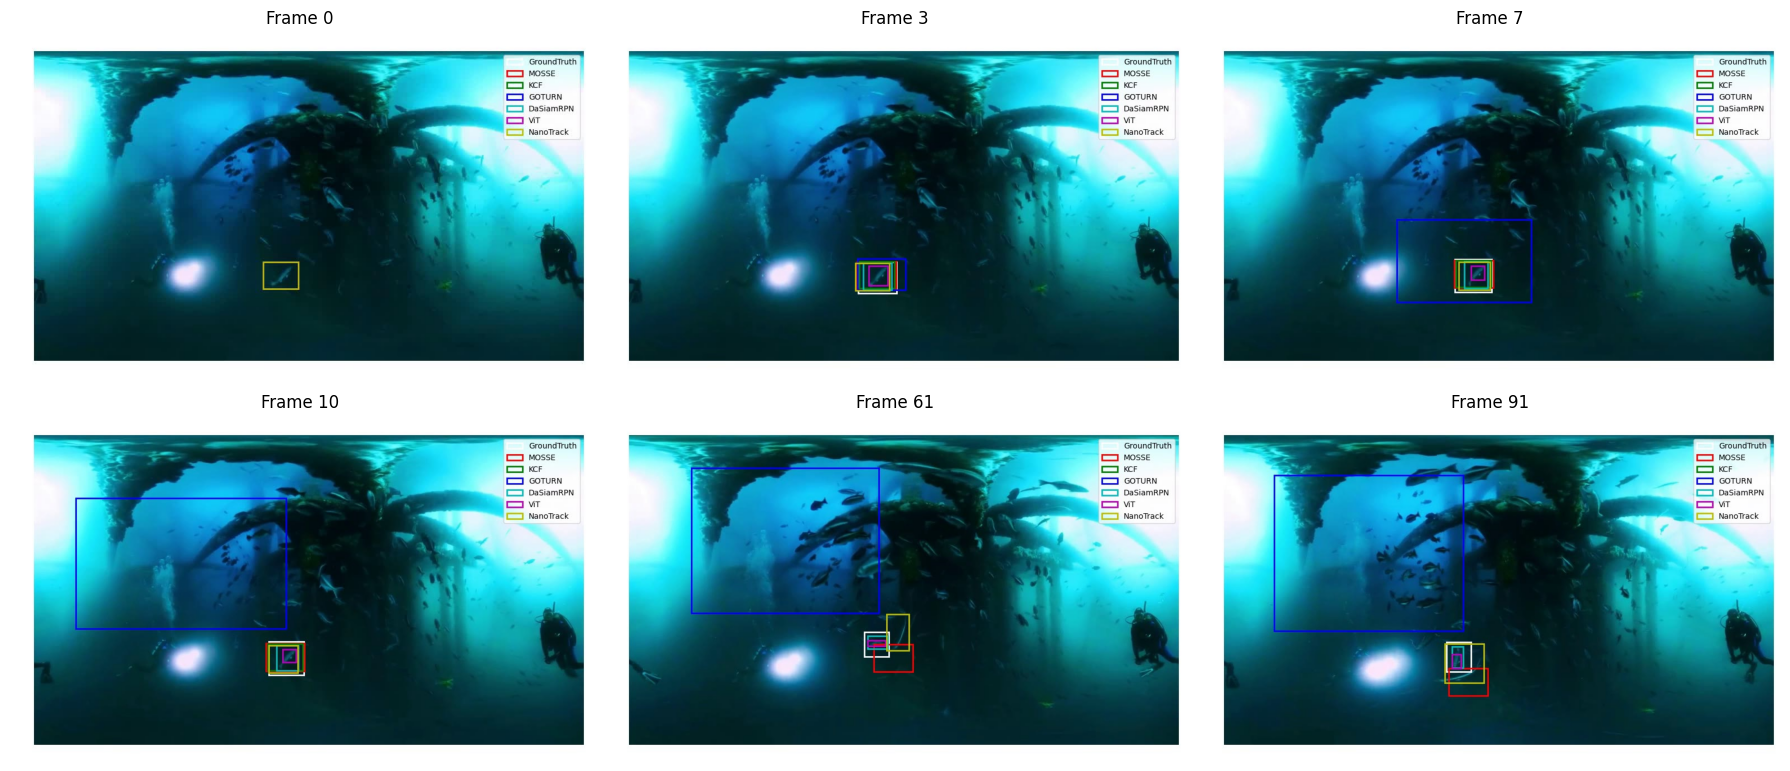
\includegraphics[width=\textwidth]{images/Diving360Degree2 copy.png}
    \caption{Tracking results on a sequence with dynamic background elements, including a school of fish and flickering illumination in a dark environment.}
    \label{fig:dynamic_bg_example}
\end{figure}

As illustrated in Figure~\ref{fig:dynamic_bg_example}, dynamic background elements severely affect tracking performance. In this sequence, ViT and DaSiamRPN exhibit the most robust tracking behavior, maintaining focus on the target despite strong distractors and illumination changes. NanoTrack, while initially performing well, loses the target at frame 61 due to confusion with background fish exhibiting similar motion and appearance.

Classical trackers such as KCF and MOSSE perform poorly in this setting, as their handcrafted features and simple update mechanisms are easily misled by background motion and lighting artifacts. Similarly, GOTURN fails to maintain consistent tracking, likely due to its limited capability to distinguish between foreground and dynamic background in low-contrast conditions.

These results highlight the importance of robust feature extraction and context-aware modeling in handling complex underwater scenes. Trackers that leverage global attention mechanisms (e.g., ViT) or adaptive region proposal networks (e.g., DaSiamRPN) are more resilient to such challenges, making them more suitable for real-world underwater applications where background motion is inevitable.


\subsubsection{Subconclusion}
The qualitative analysis of tracking results under various underwater challenges reveals that deep learning-based trackers, particularly NanoTrack and DaSiamRPN, outperform classical methods in terms of robustness and accuracy. These trackers demonstrate superior performance in low-contrast, motion blur, occlusion, and dynamic background scenarios. However, all trackers struggle with long-term occlusion and similar-looking distractors, indicating a need for further research in these areas.


\endinput